% !TEX root = presentation_29Jun.tex

\begin{frame}{Mathematical Modelling of Human-Resource Interaction}

\begin{itemize}
	\item Macroscopic variables: 
	\begin{itemize}
		\item Resource stock (palm trees): $T$
		\item Human population size: $P$
	\end{itemize} 
	\ra Human-resource interactions (Lotka-Voltera predator-prey type)
	\item So far: Dynamics described by ordinary differential equations (ODEs)
	\begin{eqnarray*}\label{eq:ode}
		\frac{d \text{P}}{dt} & = & r_\text{P} (\text{T, P, H}(\text{P})) \ \cdot \ \text{P} \\
		\frac{d \text{T}}{dt} & = & r_\text{T} (\text{T}) \ \cdot \ \text{T} \ - \   \text{H}(\text{P}) 
	\end{eqnarray*}	
with \center{$\text{H}(\text{P})$ = harvest of population $\text{P}$; \\$r_{\rm T,P}$ = functions for rates of growth}
\end{itemize}
\end{frame}

\begin{frame}{The first model on Easter Island: \citet{Brander1998}}
%The first Model: \citeTitle{Brander1998}
\centering

%\item Population grows/decays exponentially. Consumption of the resource increases the rate
%\item Result: Slow regrowth of the palm tree vs.\ faster exponential population growth \ra Malthusian Catastrophe (a.k.a.\ `Boom-Bust')

\begin{columns} \begin{column}{0.7\textwidth}
		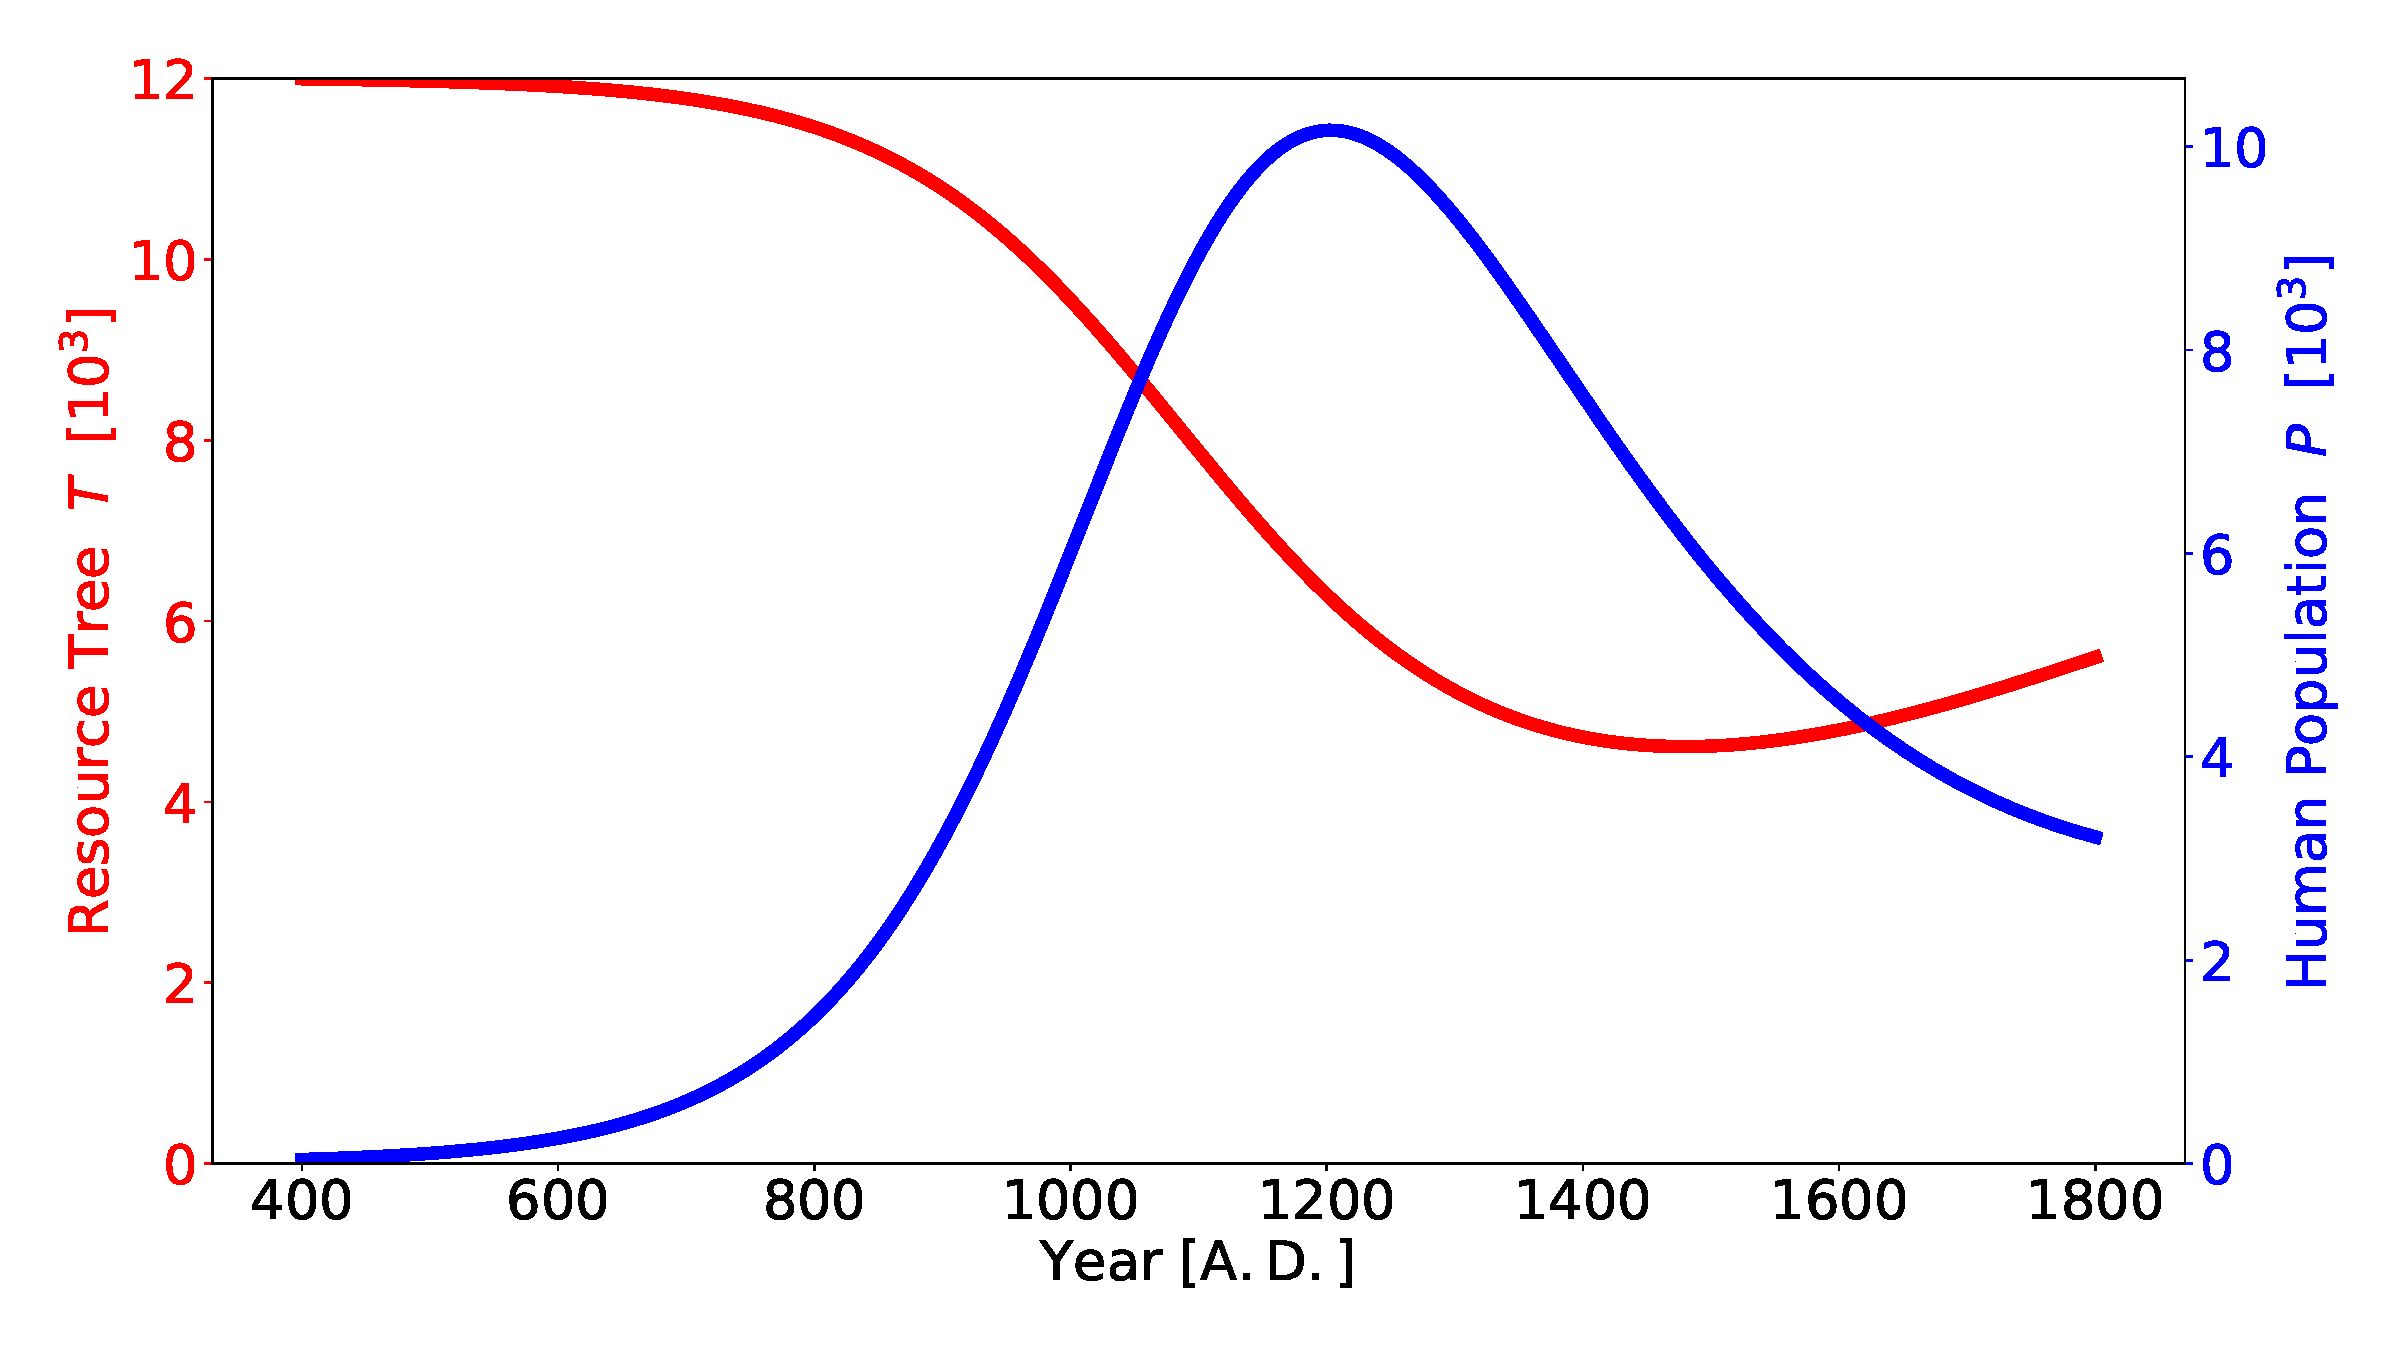
\includegraphics[width=\textwidth]{../../Thesis/images/Brander1998_EIBaseCase_presentation} 
\end{column}
\begin{column}{0.2\textwidth}
	{\footnotesize Model by \citet{Brander1998}}
\end{column}
\end{columns}
	

\begin{itemize}
\pause\item Extensions:
\begin{itemize}
	\item Socio-economic institutions \citep{Good2006}
	\item Second resource \citep{DAlessandro2007}
	\item Rat population \citep{Basener2008}
	%\item 1-dim spatial component \citep{Basener2011}
	\item Disease model \citep{Brandt2015}
\end{itemize} 
\end{itemize}                                                       
\end{frame}

\begin{frame}{Shortcomings of Dynamic System Models}
\begin{itemize}
\item Uncertainty in Parameters\\ \vspace{0.3cm}
{\centering 
	\begin{columns}
		\begin{column}{0.7\textwidth}
			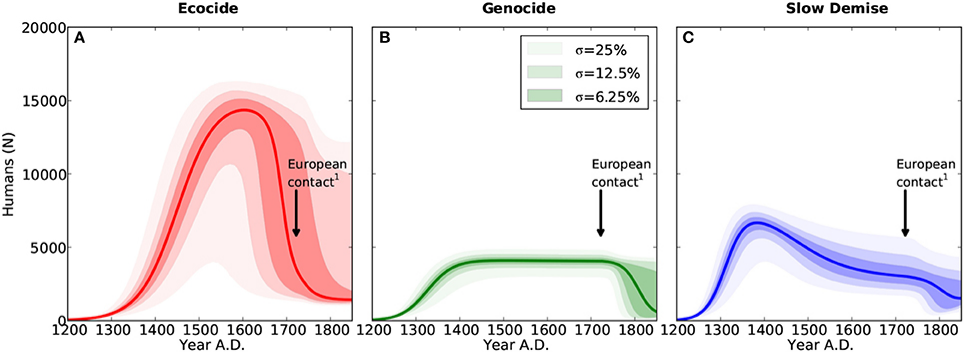
\includegraphics[width=\textwidth]{../../Brandt2015_onlyHumans}
		\end{column}
		\begin{column}{0.15\textwidth}
			{\footnotesize Model by \citet{Brandt2015}}
		\end{column}
	\end{columns}
} \vspace{0.3cm}
\ra Macroscopic view does not give insight into plausibility of resulting trajectory
\pause\item Neglect ...
\begin{itemize}
\item Spatial constraints
\item Irreducibility and heterogeneity
\item Adaptation and emergent phenomena
\item Stochasticity
\end{itemize} 
\vfill 
{\tiny More in e.g.\ \citet{Bookstaber2019}, \citet{Bonabeau2002}}
\end{itemize}
\end{frame}

